% This work is licensed under the Creative Commons
% Attribution-NonCommercial 3.0 Unported License. To view a copy of this
% license, visit http://creativecommons.org/licenses/by-nc/3.0/.

% This work is licensed under the Creative Commons
% Attribution-NonCommercial 3.0 Unported License. To view a copy of this
% license, visit http://creativecommons.org/licenses/by-nc/3.0/.

% ==========================================================================
%                     Festlegung der Dokumentenklasse
% ==========================================================================

% Dokumentklasse für Aufsätze, Berichte, etc.
\documentclass[paper=a4, german, titlepage]{scrartcl}

% Behebt ein paar Fehler in Latex
\usepackage{fixltx2e}

% ==========================================================================
%                            Detailtypographie
% ==========================================================================

\usepackage{microtype}

% ==========================================================================
%                             Zeichenkodierung
% ==========================================================================

% UTF-8 als Eingabe-Kodierung und T1 als Fontkodierung
\usepackage[utf8]{inputenc}
\usepackage[T1]{fontenc}

% ==========================================================================
%                               Schriftarten
% ==========================================================================

\usepackage{lmodern}

% ==========================================================================
%                           Spracheinstellungen
% ==========================================================================

% Deutsche Zeichenketten und deutsche Namen für die Referenzobjeke
\usepackage[german]{babel, varioref}

% ==========================================================================
%                  Aufzählungen, Referenzen und Links
% ==========================================================================

\usepackage{enumitem}

% Verlinkungen innerhalb und außerhalb des PDF-Dokuments
\usepackage{hyperref}

% Formattiert URLs, so dass sie sich z.B. besser vom Text abheben
\usepackage{url}

% TrueType-Schrift für URLs		
% \urlstyle{tt}		

% ==========================================================================
%                        Bibliograhphie und Anhang
% ==========================================================================

\newcommand{\theappendix}{
  \clearpage
  \appendix
}

% Deutsche Guillemets mit \enquote{}
\usepackage[german=guillemets]{csquotes}

\usepackage[style=numeric-comp, backend=biber]{biblatex}
\bibliography{../literatur.bib}

% Nachnamen in Kapitälchen
\renewcommand*{\mkbibnamelast}[1]{\textsc{#1}}

% ==========================================================================
%                    Grafiken, Abbildungen und Tabellen
% ==========================================================================

% Verwenden von Farben und Grafiken
\usepackage{graphicx}
\usepackage{xcolor}

% Einbinden von ganzen PDF-Seiten
\usepackage{pdfpages}

% kleine Schrift für Bildunterschriften, Fettgedruckte Bildunterschriften
\usepackage[font=small,	labelfont=bf, format=plain]{caption}

% Für mehrere Objekte nebeneinander mit eigenen Bildunterschriften
\usepackage{subcaption}

% Beinhaltet \FloatBarrier , sodass nach diesem Befehl keine Floats mehr erscheinen
\usepackage{placeins}

% Text umläuft Fließobjekte
%\usepackage{wrapfig}

% Tabellensatz
% \usepackage{tabularx}
\usepackage{booktabs}
\usepackage{longtable}

% Zum Verdrehen von Objekten. Nur mäßig verwenden.
% \usepackage{rotating}

% Setzen des Pfades für eingebundene Bilder
% \graphicspath{{figs/}{bilder/}}

% ==========================================================================
%                    Mathematikumgebungen und Einheiten
% ==========================================================================

% Paket für mathematische Umgebungen und Funktionen
\usepackage[intlimits]{amsmath}

% Zusätzliche Mathematische Schriftarten
\usepackage{amsfonts}

% Zusätzliche Mathematische Symbole
\usepackage{amssymb}

% Zum Setzen Kommutativer Diagramme
% \usepackage{amscd}

% Textsatz in der Matheumgebung
\usepackage{amstext}

% Aufrechte griechische Buchstaben
%\usepackage{upgreek}


% Diagramme mit tikz und Gnuplot zeichnen
% \usepackage{tikz}
% \usepackage{tikz-qtree}
% \usepackage{gnuplot-lua-tikz}

% ==========================================================================
%               automatischer Satz von Einheiten mit SIUnitX
% ==========================================================================

\usepackage[
% Stellt den Fehler separat dar: Siehe SIUnitX-Manual
  separate-uncertainty = true,
]{siunitx}

% Babel stellt SIUnitX auf deutsch ein, wenn german gewählt wird
\addto\extrasgerman{\sisetup{locale = DE}}

% Kürzen von Einheiten in SIUnitX ermöglichen
% \usepackage{cancel}


% ==========================================================================
%                            Textsatzparameter
% ==========================================================================

% Vermeidung von "Schusterjungen" Höchstwert 10000, dann dürfen
% theoretisch keine Schusterjungen mehr auftreten.
\clubpenalty = 3000
% Vermeidkung von "Hurenkindern" Höchstwert 10000, dann dürfen
% theoretisch keine Hurenkinder mehr auftreten.  Es werden beide
% Einstellungen benötigt.
\widowpenalty = 3000
\displaywidowpenalty = 3000


\newcommand{\name}[1]{\textsc{#1}}
\newcommand{\pdn}[3]{%
\ensuremath{\frac{\partial^{#1} #2}{\partial #3^{#1}}}}
\newcommand{\pd}[2]{%
\ensuremath{\frac{\partial #1}{\partial #2}}}
\renewcommand{\d}{\ensuremath{\mathrm{d}}}
\newcommand{\iunt}{\ensuremath{\mathrm{i}}} % imaginary unit

\titlehead{{TU Dortmund \hfill WS~14\\}
Fakultät Physik\\ Fortgeschrittenenpraktikum}

\subject{Versuchsprotokoll}
\title{Faraday-Effekt an Halbleitern}
\subtitle{Versuch 46}

\author{Daniel Meißner\\
{\normalsize\url{daniel.meissner@udo.edu}}
\and
Kevin Moch\\
{\normalsize\url{kevin.moch@udo.edu}}}

\date{16. März 2014}

\begin{document}
\maketitle

\tableofcontents
\clearpage

\section{Einleitung}

In diesem Versuch wird der Faraday-Effekt, d.h. die Drehung der 
Polarisationsachse von linear polarisiertem Licht in Materie, 
ausgenutzt, um die effektive Masse von Elektronen im Halbleiter 
GaAs zu bestimmen. 

\FloatBarrier

% This work is licensed under the Creative Commons
% Attribution-NonCommercial 3.0 Unported License. To view a copy of this
% license, visit http://creativecommons.org/licenses/by-nc/3.0/.

\section{Theorie}

\begin{figure}
  \centering
  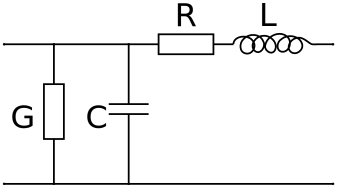
\includegraphics[scale=0.6]{ersatzschaltung}
  \caption{%
    Ersatzschaltung eines Koaxialkabels zwischen $x$ und $x + \d x$.
    Die Größen $R, L, G, C$ heißen Leitungskonstanten oder
    Leitungsbeläge.  Bei einer verlustfreien Leitung ist $R = G = 0$.
    Durch eine Betrachtung dieser Ersatzschaltung kann die
    Telegraphengleichung hergeleitet werden.}
  \label{fig:ersatz}
\end{figure}

Die Beschreibung der Ausbreitung von Signalen auf Leitungen ist
Gegenstand der Leitungstheorie.  Eine Leitung (zum Beispiel eine
Koaxialleitung, die in diesem Versuch verwendet wird) kann durch zwei
parallel verlaufende Leiter modelliert werden.  Grundaufgabe der
Leitungstheorie ist es, den zeitlichen Verlauf von Stromstärke $I(t, x)$
und Spannung $U(t, x)$ an jedem Ort $x$ der Leitung zu bestimmen.

Dazu wird ein Leitungstück von $x$ nach $x + \d x$ durch die
Ersatzschaltung aus Abbildung~\ref{fig:ersatz} dargestellt.  Die
Leitungsbeläge $R, L, G, C$ heißen auch Leitungskonstanten: $L$ und $C$
heißen Induktivitäts- bzw. Kapazitätsbelag, $R$ und $G$ heißen ohmscher
Belag bzw. Querleitfähigkeitsbelag.  Die beiden letzten kommen durch die
endliche Leitfähigkeit des Leitermaterials (Längsspannungsverluste) und
dielektrische Verlustströme zwischen der Isolierung der beiden Leiter
zustande.  Zwischen den Leitungsbelägen gibt es folgenden Zusammenhang:
%
\begin{equation}
  \label{eq:belagsformel}
  G = \frac{RC}{L}
\end{equation}

\subsection{Telegraphengleichung}

Im allgemeinen ergibt sich durch Betrachtung der Ersatzschaltung ein
System gekoppelter partieller Differentialgln. für $U$ und $I$.  Im
Falle konstanter Beläge kann dieses entkoppelt werden und es folgt eine
verallgemeinerte Wellengleichung:
%
\begin{equation}
  \label{eq:wellengl.}
  \pdn{2}{U}{x} - LC \pdn{2}{U}{t} = (LG+RC) \pd{U}{t} + RGU
\end{equation}
%
Diese Gleichung wird auch oft als Telegraphengleichung bezeichnet.  Die
Lösungen sind gedämpfte, hin- und rücklaufende harmonische Wellen:
%
\begin{equation}
  \label{eq:loesung}
  U(t, x) = U_0 \,e^{\iunt\omega t \pm \gamma x}
\end{equation}
%
Der Faktor $\gamma = \alpha + \iunt \beta = \sqrt{(R+\iunt \omega L)(G +
  \iunt \omega C)}$ heißt Ausbreitungskonstante, $\alpha$ heißt
Dämpfungsbelag und $\beta$ heißt Phasenbelag.  Die Phasengeschwindigkeit
der Welle ist daher frequenzabhängig und führt zu einer Verzerrung des
Signals.

\subsection{Leitungswellenwiderstand}

Die Art der Verzerrung wird vom Leitungswellenwiderstand beeinflußt,
welcher durch das Verhältnis von Strom- und Spannungswellen, die sich in
eine gemeinsame Richtung ausbreiten, bestimmt ist.  Für ein
sinusförmiges Signal mit der Frequenz $\omega$ ist der Wellenwiderstand
daher
%
\begin{equation}
  \label{eq:wellenwiderstand}
  Z_0 = \frac{U(\omega)}{I(\omega)} = \sqrt{\frac{R + \iunt \omega
      L}{G + \iunt \omega C}}\:.
\end{equation}
%

\subsection{Spannungs- und Strompulse}

In der Digital- und Nachrichtentechnik haben die Signale, die über eine
Leitung übertragen werden, oft die Form eines Pulses.  Die Lösungen der
entsprechenden Telegraphengleichung haben dann die Form eines hin- und
rücklaufenden Pulses, der durch die Reflexion am Leitungsende entsteht.
Der Quotient
%
\begin{equation}
  \Gamma = \frac{U_\text{r}}{U_0} = \frac{Z_\text{L} - Z_0}{Z_\text{L} + Z_0}
\end{equation}
%
heißt Reflexionsfaktor, wobei $Z_L$ hier die Lastimpedanz am Verbraucher
darstellt.  Mit seiner Hilfe kann die Form der rücklaufenden Welle aus
dem Eingangspuls berechnet werden.  Dazu wird die
\name{Laplace}-Transformation verwendet.  Sei nämlich $\tilde{U}_0(s)$
die \name{Laplace}-Transformierte der Spannung des einlaufenden und
$\tilde{U}_\text{r}(s)$ die \name{Laplace}-Transformierte der Spannung
des reflektierten Signals am Ort $x$ zur Zeit $t$, dann gilt
%
\begin{equation}
  \label{eq:reflex}
  \tilde{U}_\text{r}(s) = \Gamma\, \tilde{U}_0(s).
\end{equation}
%
Aus der Umkehrung dieser Formel unter Ausnutzung der inversen
\name{Laplace}-Transformation der zeitliche Verlauf der Spannung
$U_\text{r}(t, x)$ bestimmt werden.  Je nach Leitungsabschluß ergeben
sich hier verschiedene Signalformen.  Im Fall $Z_\text{L} = Z_0$ liegt
die sogenannte Leitungsanpassung vor, d.\,h. der Reflexionsfaktor
$\Gamma = 0$ und es gibt keine reflektierte Welle.

\subsection{Mehrfachreflexionen}

Ein Signal, das durch die Leitung läuft, wird nicht nur am Ende der
Leitung reflektiert, sondern auch am Anfang, wenn der Reflex wieder dort
ankommt.  So ergibt sich eine Reihe von Mehrfachreflexionen zwischen den
Kabelenden.  Bei jedem Reflex wird die Amplitude des Signals um einen
entsprechenden Reflexionsfaktor $\Gamma$ geschwächt.  Sei der
Reflexionsfaktor des Kabelanfangs $\Gamma_\text{a}$ und der des
Kabelendes $\Gamma_\text{e}$, dann gilt im Grenzfall unendlicher
Reflexion für die Amplitude der Signalspannung:
%
\begin{equation}
  U_\infty = U_0(1 + \Gamma_\text{e} + \Gamma_\text{a} \Gamma_\text{e}
  + \Gamma_\text{a} \Gamma_\text{e}^2 + \Gamma_\text{a}^2
  \Gamma_\text{e}^2 + \dotsb) = U_0 \:\frac{1 + \Gamma_\text{e}}{1
    - \Gamma_\text{a} \Gamma_\text{e}}
\end{equation}
%

Befinden sich im Kabel zusätzlich Störstellen (z.\,B. wenn zwei
verschiedene Kabel aneinander gesteckt sind), gibt es auch an diesen
Stellen Reflexionen.  Um den Überblick zu behalten, kann es in solchen
Fällen hilfreich sein, einen sogenannten Impulsfahrplan anzufertigen.
In Abschnitt~\ref{sec:durchfuehrung-mehrfachreflexion} wird eine
Situationen, in der zwei unterschiedliche Kabel verbunden sind,
beschrieben.

\subsection{Ausgewählte Leitungsabschlüsse}

In diesem Abschnitt werden die Signalverläufe zu drei verschiedenen
Abschlußwiderständen berechnet.  Die erhaltenen Funktionen werden später
verwendet, um eine Ausgleichsrechnung mit den aufgenommenen Meßwerten
durchzuführen.  Der einlaufende Signalverlauf\footnote{Die Amplitude
  wird hier auf 1 normiert, um die Rechnungen nicht zu überladen.  Da
  die \name{Laplace}-Transformation eine lineare Abbildung ist, kann ein
  Faktor für die Amplitude nachträglich hinzugefügt werden.}  kann mit
der \name{Heaviside}-Funktion~$\Theta$ so geschrieben werden:
%
\begin{equation}
  U_0(t) = \Theta(t).
\end{equation}
%
Die \name{Laplace}-Transformierte lautet dann $\tilde{U}_0(s) = s^{-1}$.
Mit Formel~\eqref{eq:reflex} wird daraus durch Rücktransformation der
Reflex am Leitungsende berechnet.

\paragraph{Abschluß durch Induktivität} Im Falle einer Induktivität als
Abschluß ist $Z_\text{L} = \iunt\omega L$ und damit ergibt sich für $s =
\iunt\omega$ der Reflexionsfaktor zu
%
\begin{equation}
  \Gamma = \frac{sL - Z_0}{sL + Z_0} = \frac{s - \tau^{-1}}{s + \tau^{-1}}
\end{equation}
%
mit $\tau := L/Z_0$. Jetzt wird gemäß Formel~\eqref{eq:reflex} das
reflektierte Signal berechnet.  Zerlege dazu $\Gamma \tilde{U}_0(s)$ in
Partialbrüche:
%
\begin{equation}
  \tilde{U}_\text{r}(s) = \Gamma\tilde{U}_0(s) = \frac{s - \tau^{-1}}{s(s
    + \tau^{-1})} = \frac{2}{s + \tau^{-1}} - \frac{1}{s}
\end{equation}
%
Nach den Eigenschaften der \name{Laplace}-Transformation bezüglich
Translation das reflektierte Signal für $t>0$ erhalten:
%
\begin{equation}
  \label{eq:ind_reflex}
  U_\text{r}(t) = 2e^{-\frac{t}{\tau}} - 1.
\end{equation}

\paragraph{Abschluß durch Induktivität und ohmschen Widerstand} In
diesem Fall wird $Z_\text{L} = R + \iunt \omega L$ und der
Reflexionsfaktor lautet
%
\begin{equation}
  \Gamma = \frac{R + sL - Z_0}{R + sL - Z_0} = \frac{s + (R-Z_0)L^{-1}}{s + \tau^{-1}}
\end{equation}
%
mit $\tau := L/(Z_0 + R)$.  Jetzt wird analog zu oben verfahren.  Eine
Partialbruchzerlegung von $\Gamma \tilde{U}_0(s)$ liefert:
%
\begin{equation}
  \tilde{U}_\text{r} (s) = \Gamma \tilde{U}_0(s) = \frac{s + (R -
    Z_0)L^{-1}}{s(s + \tau^{-1})} = \frac{\Gamma_0}{s} + \frac{1
    - \Gamma_0}{s + \tau^{-1}}
\end{equation}
%
mit $\Gamma_0 := \frac{R - Z_0}{R + Z_0}$.  Daraus wird das reflektierte
Signal durch Rücktransformation erhalten:
%
\begin{equation}
  \label{eq:ind_ohm_reflex}
  U_\text{r}(t) = \Gamma_0 + (1 - \Gamma_0) e^{-\frac{t}{\tau}}.
\end{equation}

\paragraph{Abschluß durch Kapazität und ohmschen Widerstand} Hier ist
$Z_\text{L} = R + \frac{1}{\iunt \omega C}$ und der Reflexionsfaktor
lautet dann:
%
\begin{equation}
  \Gamma = \frac{\frac{1}{sC} + R - Z_0}{\frac{1}{sC} + R + Z_0}
  = \frac{\Gamma_0 s + \tau^{-1}}{s + \tau^{-1}} 
\end{equation}
%
mit $\Gamma_0$ wie oben und $\tau := (R+Z_0) C$.  Nach der
Partialbruchzerlegung
%
\begin{equation}
  \Gamma \tilde{U}_0(s) = \frac{1}{s} + \frac{\Gamma_0 - 1}{s + \tau^{-1}}
\end{equation}
%
lautet nach Rücktransformation das reflektierte Signal so:
%
\begin{equation}
  \label{eq:cap_ohm_reflex}
  U_\text{r}(t) = 1 + (\Gamma_0 - 1) e^{-\frac{t}{\tau}}.
\end{equation}

% This work is licensed under the Creative Commons
% Attribution-NonCommercial 3.0 Unported License.  To view a copy of
% this license, visit http://creativecommons.org/licenses/by-nc/3.0/.

\section{Durchführung}
%
Im gesamten Versuch wird die in Abb.~\ref{fig:aufbau} schematisch 
dargestellte Schaltung zum Durchführen der Messungen verwendet.
%
\begin{figure}
  \centering
  \includegraphics[width=0.7\textwidth]{aufbau}
  \caption{Der schematische Schaltplan, mit dem die Impulse
               des Zählrohres gemessen werden können. Außerdem zu sehen 
                ist ein Strommessgerät und ein Oszilloskop.
                 Die Skizze wurde aus \textcite{v703} entnommen.}
  \label{fig:aufbau}
\end{figure}
%
\subsection{Messung der Charakteristik und pro Teilchen freigesetzte Ladungsmenge}
%
Zur Messung der Charakteristik des Geiger-Müller-Zählrohres wird für
\num{14} verschiedene Spannungen zwischen Anodendraht und
Kathodenmantel, welche von \SI{320}{\volt} bis \SI{700}{\volt}
eingestellt werden, die Impulsanzahl und die Stromstärke gemessen.
Dabei werden die Impulse in einer Zeitspanne von je \SI{120}{\second}
gezählt.

Die hierbei verwendete $\beta$-Strahlenquelle wird in einem solchen
Abstand eingesetzt, dass bei einer angelegten Spannung von
\SI{320}{\volt} ca. \num{100} Impulse pro Sekunde gemessen
werden. Dadurch sollen Totzeitkorrekturen vermieden werden.  Die
Stromstärkemessung dient der Ermittlung der freigesetzen Ladungsmenge
pro registriertem Teilchen. In Formel~\eqref{eq:ladungsmenge} ist der
Zusammenhang zwischen gemessener Stromstärke $I$, Ladungsmenge $Q$ und
Teilchenzahl pro Zeit $\frac{Z}{\Delta t}$ angegeben.
\begin{equation}
I = \frac{Z}{\Delta t} Q
\label{eq:ladungsmenge}
\end{equation}
%
\subsection{Nachentladungszeitmessung}
%
Diese Messung wird mithilfe des in Abb.~\ref{fig:aufbau} gezeigten
Oszilloskops durchgeführt. Die Ablenkgeschwindigkeit des Kathodenstrahls
wird hierbei so eingestellt, dass ein Zentimeter, bzw. ein Kästchen,
einer Zeit von \SI{50}{\micro\second} entspricht. Das Oszilloskop wird
mit der Anstiegsflanke der Zählrohrimpulse getriggert.

Die Strahlungsquelle wird bei \SI{350}{\volt} in einer solchen
Entfernung zum Zählrohr angebracht, dass neben dem durch ein
registriertes Teilchen hervorgerufenen Impuls kein, oder kaum ein,
weiteres Teilchen während der Auslenkung des Kathodenstrahls über den
gesamten Oszilloskopenschirm registriert wird.

Nun wird die Spannung auf \SI{700}{\volt} erhöht, sodass es zu
Nachentladungen kommt.  Am Oszilloskop wird nun der Abstand zwischen
Primär- und Nachentladungspeak abgelesen.
%
\subsection{Totzeitmessung}
Um die Totzeit des verwendeten Zählrohres zu bestimmen werden in diesem
Versuch zwei Methoden verwendet, die nun präsentiert werden.
\subsubsection{Mit einem Oszilloskop}
%
Die Totzeitbestimmung mithilfe eines Oszilloskops verläuft beinahe
analog zur Nachentladungszeitmessung. Bei der Totzeitmessung wird
allerdings die Strahlenquelle so nahe wie möglich an das Zählrohr
angebracht, um eine hohe Strahlenintensität im Zählrohr zu erhalten.

Bei \SI{700}{\volt} Spannung am Zählrohr wird das getriggerte
Oszilloskopenbild betrachtet. An diesem wird nun abgelesen, ab welcher
Zeit nach dem Registrieren eines Teilchen das Zählrohr wieder zum
Erzeugen eines Impulses fähig ist.

Es wird hierbei auch direkt eine Messung zur Erholungszeit des
Zählrohres durchgeführt.  Dazu wird die interne Zeitablenkung auf
\SI{100}{\micro\second} erhöht, um festzstellen, ab wann wieder die
ursprüngliche Impulshöhe erreicht wird.
%
\subsubsection{Mit der Zwei-Quellen-Methode}
%
Bei der Zwei-Quellen-Methode werden drei Messungen durchgeführt.  Als
erstes wird eine Quelle 1 so nah wie möglich an das Zählrohr angebracht,
woraufhin bei einer angelegten Spannung von \SI{500}{\volt} die vom
Zählrohr in einer Zeitspanne von \SI{180}{\second} registrieren Impulse
gezählt werden.

Anschließend wird eine weiter Quelle 2 vor das Zählrohr gesetzt, sodass
die Strahlung beider Quellen registiert werden kann. Die Messung, welche
bei Quelle 1 durchgeführt wurde, wird wiederholt.  

Zum Schluss wird Quelle 1 entfernt, sodass nur noch die von Quelle 2
emittierten Teilchen vom Zählrohr registriert werden. Die Messung wird
ein weiteres mal wiederholt.  Aus den erhaltenen Impulsen und der
Messzeit lassen sich nun die registierten Impulse pro Zeit $N_1$ für
Quelle 1, $N_2$ für Quelle 2 und $N_{1+2}$ für beide Quellen zusammen
errechnen. Mit Formel~\eqref{eq:zwei_quellen} wird nun die Totzeit des
Zählrohres bestimmt.
%
\begin{equation}
\frac{N_{1+2}}{1- TN_{1+2}} = \frac{N_1}{1 - TN_1} + \frac{N_2}{1- TN_2}
\label{eq:zwei_quellen}
\end{equation}
%
Gilt $1 \gg T^2N_i^2$, so kann Formel~\eqref{eq:zwei_quellen} auch zu
Formel~\eqref{eq:zwei_quellen_naeherung} genähert werden.
%
\begin{equation}\label{eq:zwei_quellen_naeherung}
  T \approx \frac{N_1 + N_2 - N_{1+2}}{2N_1N_2}
\end{equation}

\FloatBarrier


% Literaturverzeichnis
\addcontentsline{toc}{section}{Literatur}
\printbibliography
% Anleitung auf jeden Fall zitieren
\nocite{v046}

\theappendix

\end{document}
